\documentclass{article} \usepackage{amsmath} \usepackage{amssymb} \usepackage{amsthm} \usepackage[margin=0.2in]{geometry} \usepackage{hyperref} \usepackage{physics} \usepackage{tikz} \usepackage{mathtools} \mathtoolsset{showonlyrefs} \theoremstyle{definition} \newtheorem{theorem}{Theorem}[section] \newtheorem{corollary}{Corollary}[theorem] \newtheorem{lemma}[theorem]{Lemma} \newtheorem{definition}{Definition}[section] \author{Connor Duncan} \date{\today}
\title{Physics-105-Lecture-Notes-04-09-2019}
\begin{document}
\maketitle\tableofcontents
\noindent\abstract{A single PDF with all lectures in a single document can be downloaded at \url{https://www.dropbox.com/sh/8sqzvxghvbjifco/AAC9LoSRnsRQDp7pYedgWpQMa?dl=0}. The password is 'analytic.mech.dsp'.
 This file was automatically generated using a script, so there might be some errors. If there are, you can contact me at \url{mailto:ctdunc@berkeley.edu}.}
\section{Small Oscillations} \subsection{Stationary Points} Consider a lagrangian $\mathcal L=\frac{1}{2}m\dot x^2-V(x)$, with generalized coordinates $(x,\dot x)$. Recall ELE \begin{equation} \dv{t}\left(\pdv{\mathcal L}{\dot x}\right)=\pdv{\mathcal L}{x} \end{equation} a stationary point is a point $x_0$ such that $\dot x_0=0\Rightarrow=x_0\forall t$, which gives that $\pdv{V}{x}=0$. It's a point with no force acting on a system. \paragraph{mass on spring} A mass on a spring (simple harmonic oscillator) has potential $V(x)=\frac{1}{2}k(x-x_*)^2$, which looks as \begin{center} 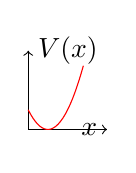
\begin{tikzpicture} \draw[->] (0,0)--(1,0) node[anchor=east]{$x$}; \draw[->] (0,0)--(0,1) node[anchor=west]{$V(x)$}; \draw[smooth,domain=0:0.7,variable=\x,red] plot({\x},{(2*\x-0.5)^2}); \end{tikzpicture} \end{center} at those stationary points, there are small oscillations that we can taylor expand to have that \begin{equation} \begin{matrix} m\delta\ddot x=-\dv[2]{V}{x}_{x=x_i}\delta x\\ \delta x=Ae^{-i\omega t}\\ \omega^2=\frac{1}{m}\dv[2]{V}{x}_{x=x_i} \end{matrix} \end{equation} The most general expression for a lagrangian is \begin{equation} \mathcal L(q,\dot q)=T(q,\dot q)-V(q) \end{equation} with \begin{equation} T=\frac{1}{2}\sum T_{ik}\dot q_i\dot q_k \end{equation} or, in other words \begin{equation} T=\frac{1}{2}\sum_im_i|\dot{\vec{r_i}}|^2 \end{equation} which allows some reexpression of $T$ as \begin{align} T=\frac{1}{2}\sum_{i,\alpha\beta}m_i\pdv{\vec{r_i}}{q_\alpha}\pdv{\vec{r_i}}{q_\beta}\dot q_\alpha\dot q_\beta\\ =\frac{1}{2}\sum_{\alpha,\beta}\left[\sum_im_i\pdv{\vec{r}_i}{q_\alpha}\pdv{\vec{r}_i}{q_\beta}\right]\dot q_\alpha\dot q_\beta \end{align} if we wanted to write this down as a symmetric tensor ($T_{ij}=T_{ji}$), then we should take some kinetic energy of the form \begin{equation} T=\frac{1}{2}(T_{11}\dot q_1^2+T_{12}\dot q_1\dot q_2+T_{21}\dot q_1\dot q_2+T_{2@}\dot q_2^2) \end{equation} and reexpress it as \begin{equation} T=\frac{1}{2}(T_{11}\dot q_1^2+\frac{T_{12}+T_{21}}{2}\dot q_1\dot q_2+\frac{T_{12}+T{21}}{2}\dot q_2\dot q_1+T_{22}\dot q_2^2) \end{equation} For a more abstrat system, for a stationary point $q^0$ where the superscript denotes stationary status, not exponentiation, we have that $\dot q_k=0$ for ever $k$ index, and that $\pdv{V}{q_\alpha}=0\forall \alpha\in$ our range. For the case where $T_{ik}$ depends on $q$, then our lagrangian is \begin{align} \mathcal L=\frac{1}{2}\sum_{i,k}T_{ik}(q)\dot q_i\dot q_k-V(q) \end{align} which we can apply standard ops to to derive that \begin{align} \dv{t}\left[\sum_kT_{\alpha k}\dot q_k\right]=\frac{1}{2}\sum_{i,k}\pdv{T_{ik}}{q_\alpha}\dot q_i\dot q_k-\pdv{V}{q_\alpha} \end{align} the final form comes out to be \begin{equation} \sum_k T_{\alpha k}\ddot q_k=-\pdv{V}{q_\alpha}+\frac{1}{2}\sum_{i,k}\pdv{T_{ik}}{q_\alpha}\dot q_i\dot q_k-\sum_{k,s}\pdv{T_{\alpha k}}{q_s}\dot q_s\dot q_k \end{equation} which are newtons equations for this lagrangian. Now, we are considering the behavior of a system around a stationary point in $n$ generalized coordinates. We take the lagrangian and expand \begin{align} \mathcal L=\frac{1}{2}\sum_{i,k}T_{ik}(q)\dot q_i\dot q_k-V(q_i) \end{align} if we expand up to quadratic terms, we are taking \begin{equation} \mathcal L=\frac{1}{2}\sum_{i,k}T_{ik}(q^{(0)}+\delta q)\delta\dot q_i\delta\dot q_k-V(q^{(0)}-\sum_i\pdv{V}{q_i}_0\delta q_i-\frac{1}{2}\sum_{i,j}\pdv[2]{V_{ij}}{q_i}{q_j}\delta q_i\delta q_j \end{equation} Constant terms we set to zero, and we get that (setting the mass tensor $T_{ik}(q^{(0)}=m_{ik}$ and $V_{ij}$ another tensor whos name i forget, we have \begin{equation} \mathcal L=\frac{1}{2}\sum_{i,k}m_{ik}\dot q_i\dot q_k-\frac{1}{2}\sum_{ik}V_{ik}q_iq_k \end{equation} in a single equation, we just end up with $m\ddot x=-kx$ which is what we expect. This is apparently pretty easy in particular systems, so let's take a look at an example. \subsubsection{Example: Coupled Pendulum} Consider two identitical masses connected by two identical ropes, ith generalized coordinates $\phi_1,\phi_2$, in a cartesian $x,y$ system. So, \begin{align} x_1 = e\sin\phi_1 && y_1=-e\cos\phi_1 \\ x_2=e\sin\phi_1+e\sin(\phi_1+\phi_2) && y_2=-e\cos\phi_1-e\cos(\phi_1+\phi_2) && \end{align} With the conclusion that \begin{equation} T_1=\frac{1}{2}ml^2\dot\phi_1^2 \end{equation} and \begin{equation} T_2=\frac{1}{2}m[l^2\dot\phi_1^2+l^2(\dot\phi_1+\dot\phi_2)^2+2l^2\dot\phi_1(\dot\phi_1+\dot\phi_2)\cos\phi_2] \end{equation} The total kinetic energy then, is (after a lot of algebraic simplification \begin{equation} T=\frac{1}{2}ml^2\left[2\dot\phi_1^2+(\dot\phi_1+\dot\phi_2)^2+2\dot\phi_1(\dot\phi_1+\dot\phi_2)\cos\phi_2\right] \end{equation} Potential energy is given by \begin{align} V=-mgl\cos\phi_1-mg(l\cos\phi_1+l\cos(\phi_1+\phi_2)\\ =-mgl(2\cos\phi_1+\cos(\phi_1+\phi_2) \end{align} So we want \begin{equation} \pdv{V}{\phi_1}=0\Rightarrow\sin(\phi_1)+\sin(\phi_1+\phi_2)=0 \end{equation} If we want to standardize our kinetic energy, we should rewrite it as \begin{align} T=\frac{1}{2}ml^2[2\dot\phi_1^2+\dot\phi_1^2+2\dot\phi_1\dot\phi_2+\dot\phi_2^2+2\dot\phi_1^2\cos\phi_2+2\dot\phi_1\dot\phi_2\cos\phi_2]\\ =\frac{1}{2}ml^2[(3+2\cos\phi_2)\dot\phi_1^2+\dot\phi_2^2+2\dot\phi_1\dot\phi_2(1+\cos\phi_2)] \end{align} which gives \begin{align} T_{11}=(3+2\cos\phi_2)ml^2\\ T_{12}=T_{21}=(1+\cos\phi_2)ml^2\\ T_{22}=ml^2 \end{align} Now, we have to expand the system, so that \begin{align} V=-mgl\left[ \left( 1-\frac{\phi_1^2}{2} \right)2 + \left( 1-\frac{(\phi_1+\phi_2)^2}{2} \right) \right] \\ V=\frac{1}{2}mgl[2\phi_1^2+(\phi_1+\phi_2)^2]=\frac{1}{2}mgl[3\phi_1^2+2\phi_1\phi_2+\phi_2^2] \end{align} when we ignore constants, which is allowable because of the lagrangian formalism. Kinetic energy about our expansion goes as \begin{align} \frac{1}{2}ml^2\left[ 5\dot\phi_1^2+4\dot\phi_1\dot\phi_2+\dot\phi_2^2 \right] \end{align} Finally, this gives us the lagrangian \begin{equation} \mathcal L=\frac{1}{2}ml^2\left( 5\dot\phi^2_1+4\dot\phi_1\dot\phi_2+\dot\phi_2^2 \right) -\frac{1}{2}mgl(3\phi_1^2\phi_1\phi_2+\phi_2^2) \end{equation} which means we can write down \begin{align} m_{ik}=\begin{bmatrix} 5 & 2\\ 2 & 1 \end{bmatrix} \\ V_{ik}=\begin{bmatrix} 3 & 1\\ 1 & 1 \end{bmatrix}\omega_0^2 \end{align} where $\omega_0^2=g/l$. This just gives us a solution of the form $q_k=A_ke^{-i\omega t}$, which we know how to solve. \begin{equation} -\omega^2m_{\alpha k}+V_{\alpha k})A_k=0 \end{equation} which is a statement about whether or not the solution has nontrivial solutions, i.e. it only does if \begin{equation} \det(\hat V-\omega^2\hat m)=0 \end{equation} Now, let's try taking \begin{align} \sum_{ik}A_{i}^{(s)}(V_{ik}-\omega_{s}^2m_{ik})A_k^{(s)}=0\Rightarrow \omega_S^2=\frac{V_{ik}A_i^{(s)}A_k^{(s)}}{m_{ik}A_i^{(s)}A_k^{(s)}} \end{align} We now want to solve \begin{align} \det\left( \begin{bmatrix} 3\omega_0^2-5\omega^2 & -\omega_0^2-2\omega^2\\ \omega_0^2-2\omega^2 & \omega_0^2-\omega^2 \end{bmatrix} \right) \end{align} which gives a characterisitc equation \begin{equation} \omega^4-4\omega^2\omega_0^2+2\omega_0^2=0 \end{equation} which gives that \begin{equation} \omega_1^2=\omega_0^2(2+\sqrt{2}) \end{equation} and \begin{equation} \omega_2^2=\omega_0^2(2-\sqrt{2}) \end{equation} and then we find the eigenvectors of this matrix using usual linear algebra methods.
\end{document}
